A Dyck $n$-path is a lattice path of  $n$  upsteps $(1,1)$ and  $n$
  downsteps $(1,-1)$
that starts at the origin  $O$  and never dips below the  $x$-axis.
A return is a maximal sequence of contiguous downsteps that terminates
on the  $x$-axis. For example, the Dyck 5-path illustrated has two returns,
of length  3  and  1  respectively.
\begin{center}
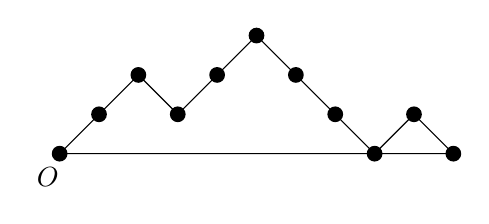
\begin{tikzpicture}[scale=.5]
\fill (0,0) circle (.2); \fill (1,1) circle (.2); \fill (2,2) circle (.2);
\fill (3,1) circle (.2); \fill (4,2) circle (.2); \fill (5,3) circle (.2);
\fill (6,2) circle (.2); \fill (7,1) circle (.2); \fill (8,0) circle (.2);
\fill (9,1) circle (.2); \fill (10,0) circle (.2);
\draw (0,0) -- (2,2) -- (3,1) -- (5,3) -- (8,0) -- (9,1) -- (10,0) -- cycle;
\draw (-.3,-.1) node[anchor=north] {$O$};
\end{tikzpicture}
\end{center}
Show that there is a one-to-one correspondence between the Dyck  $n$-paths
with no return of even length and the Dyck $(n-1)$-paths.
